\chapter{Graded membership strategy}
\label{s:graded-operators}

As in the previous chapter for the basic colour strategy, the
implementation of the graded membership strategy can be
completed by defining its adoption, alignment and invention
operator. Instead of inventing and acquiring colour categories, the
graded membership strategy allows agents to invent and acquire
membership categories. The invention operator allows users to expand
the current language system with a new membership category and a new
lexical rule to express this category in language whenever they feel
the current system is insufficient for their communicative needs. The
adoption operator allows users to pick up these newly invented terms
and the corresponding membership categories. The alignment operator
specifies how language users can align the prototypical values of the
membership categories they are using.

\section{Adoption and alignment operators}

The main goal of the adoption and alignment operators of the graded
membership strategy, is to ensure that an agent can acquire the
membership categories of another agent. The learner needs to be able
to figure out how many membership categories are used by the other
agent, and what the prototypical membership values of these categories
are.

The adoption operator 
\is{learning operators!adoption operator!for graded membership strategy}
of the graded membership strategy is triggered
whenever an agent hears an unknown term in combination with a known
term which is associated with a colour category. The agent determines
the membership value of the colour of the topic to the interpreted colour
category and learns a new membership category based on this 
value. The resulting membership category is associated with the
previously unknown term.

After each interaction in which a membership category is used, the
alignment operator
\is{learning operators!alignment operator!for graded membership strategy}
for the graded membership strategy is
used to ensure the prototypical membership values become aligned between agents. This
operator involves determining the membership value of the current
topic to the colour category used and adapting the membership value of the
used membership category to this value. The rate at which this
alignment happens is based on the \textsc{membership category alignment rate},
\is{alignment rate!membership category}
\is{membership category alignment rate|see{alignment rate}}
which linearly
determines how much the prototypical value of the membership category
should be adapted to the current situation. In this chapter, the membership category
alignment rate is set to 0.05 unless stated otherwise.

\subsection{Acquisition experiment}
\is{acquisition experiment!for graded membership strategy}

In the acquisition experiment, one agent needs to learn the membership
categories used by another agent through interactions based on a set
of shared basic colour categories. These membership categories are
identical to the ones used in the baseline experiment of the
graded membership strategy for Tarahumara as described in
Section \ref{s:gms-baseline-experiment}. The contexts about which the
agents have to communicate consist of five randomly chosen Munsell
chips \citep{newhall42final}, without any additional constraints.

\subsection{Measures}

\subsubsection{Membership category variance}
\is{measures!membership category variance}
\is{membership category variance|see{measures}}

The membership category variance is defined similarly to the
interpretation variance for basic colour categories, but instead of
computing the distance between the different colour categories in a
conceptual space, the difference between the prototypical values of
the membership categories is used in this measure. The lower the
variance, the higher the coherence between the membership categories
of the agents.

For each unique form ($f$) that is associated with a membership category
in a population of agents $P$, the membership category variance is
computed with in the subset $A_f = \{a_1, a_2, ..., a_n\}$ of agents
that know this form, as shown in Equation \ref{eq:mcv-form}. For each
pair of agents the difference between the prototypical values of the
membership categories is computed and averaged.

\begin{equation}
I_{mcv}(f) = \frac{2}{n(n-1)} \sum^n_{i=1} \sum^n_{j=i+1} d(a_i(f), a_j(f))
\label{eq:mcv-form}
\end{equation}

Following an identical reasoning as for the interpretation variance,
the formula for computing the membership category variance for all
forms ($F$) that are associated with a membership category within a
population, is defined in Equation \ref{eq:mcv-population}, where
$|P|$ is the population size and $|a_i|$ is the total number of forms
that are known to agent $a_i$.

\begin{equation}
  I_{mcv}(P) = \sum_{f \in F} \left(\sum_{i=1}^{n} \frac{1}{|P||a_i|}\right) I_{mcv}(f)
\label{eq:mcv-population}
\end{equation}

\subsection{Results}

The resulting dynamics are shown in Figure
\ref{f:gm-acquisition-dynamics}. Initially, the communicative success
of the learner is lower than the baseline communicative success. This is due to the
initial guesses made by the learner on the prototypical membership values of the 
membership categories used by the teacher. After some interactions, the
alignment of the membership categories improves, as shown by a
decrease in the membership category variance measure. This is
also reflected by an increase of the communicative success of the learner
which in the end of the experiment matches the baseline communicative
success. The number of membership categories known to the learner is
not shown, as this would obscure the details of the membership
category variance, but in each run the learner quickly picks up the three different
membership categories used by the teacher.

\begin{figure}[htpb]
  \begin{center}
    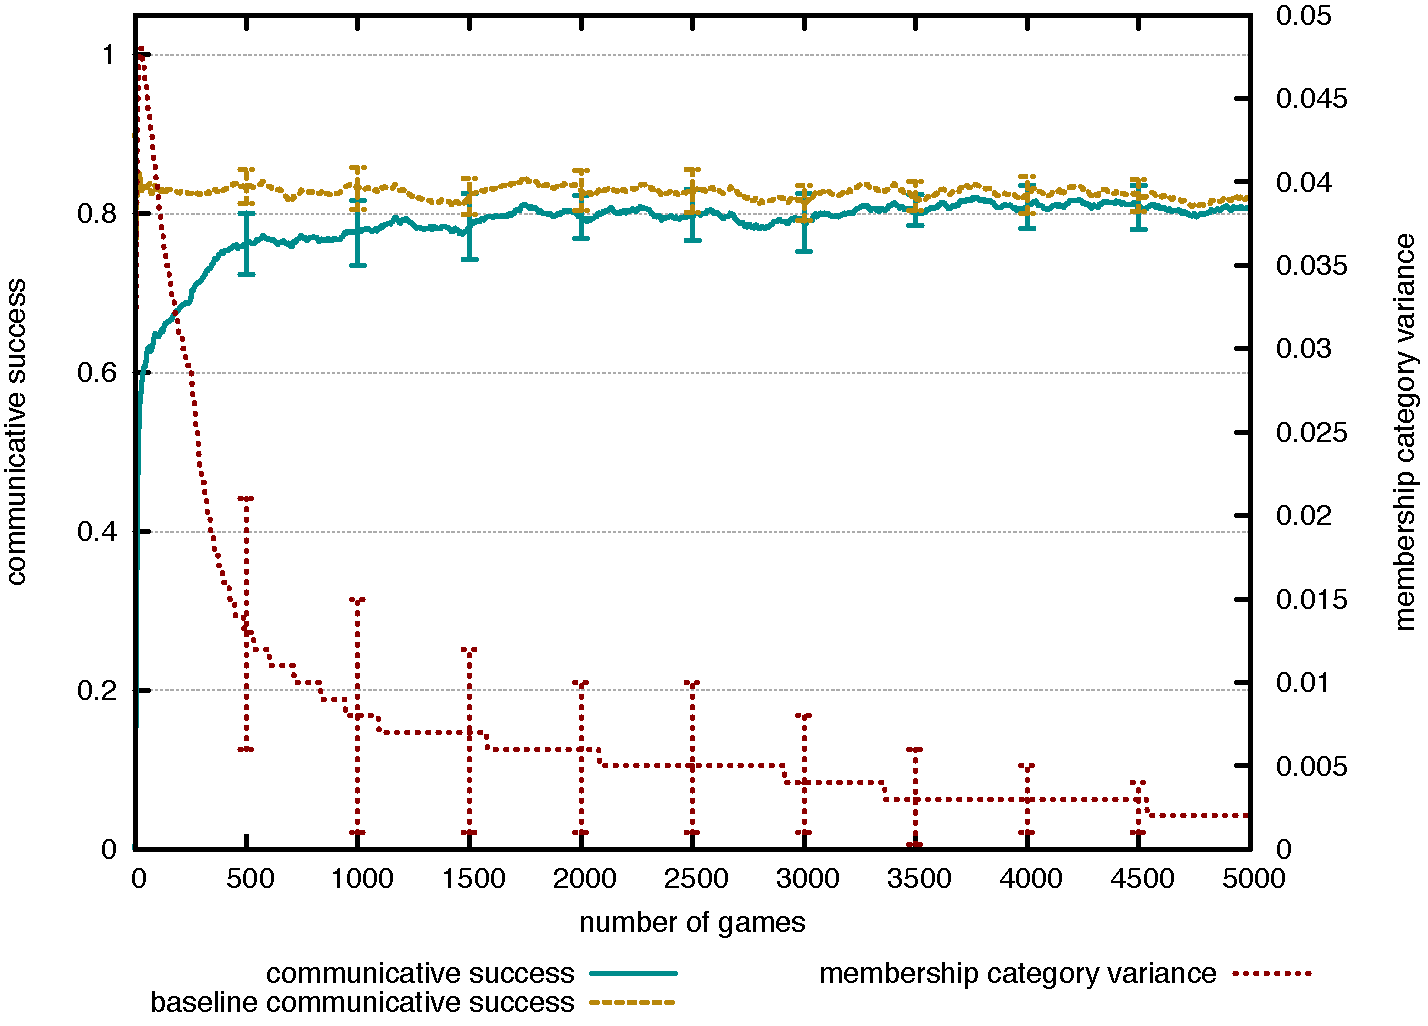
\includegraphics[width=.8\textwidth]{./graded-membership/figures/strict-acquisition.pdf}
    \caption[Dynamics of the acquisition experiment for the graded
    membership strategy]{Dynamics of the acquisition experiment for
      the graded membership strategy. The learner is able to pick up
      the membership categories used by the teacher, as shown by its
      communicative success. This success matches the baseline communicative
      success as the membership category variance decreases. The
      results are averaged over 10 independent runs.}
    \label{f:gm-acquisition-dynamics}
  \end{center}
\end{figure}

Another way of verifying the performance of the adoption and alignment
operators is by tracking the prototypical membership values of the
categories known to the learner over time. An example of a graph tracking these values
is shown in Figure \ref{f:gm-acquisition-values} and the target values
are shown in Table \ref{t:gms-tarahumara-modifiers}. Although the
initial guesses of the prototypical values are quite different from
the target values, the alignment operator enables the agent to learn
the correct values over time.

\begin{figure}[htpb]
  \begin{center}
    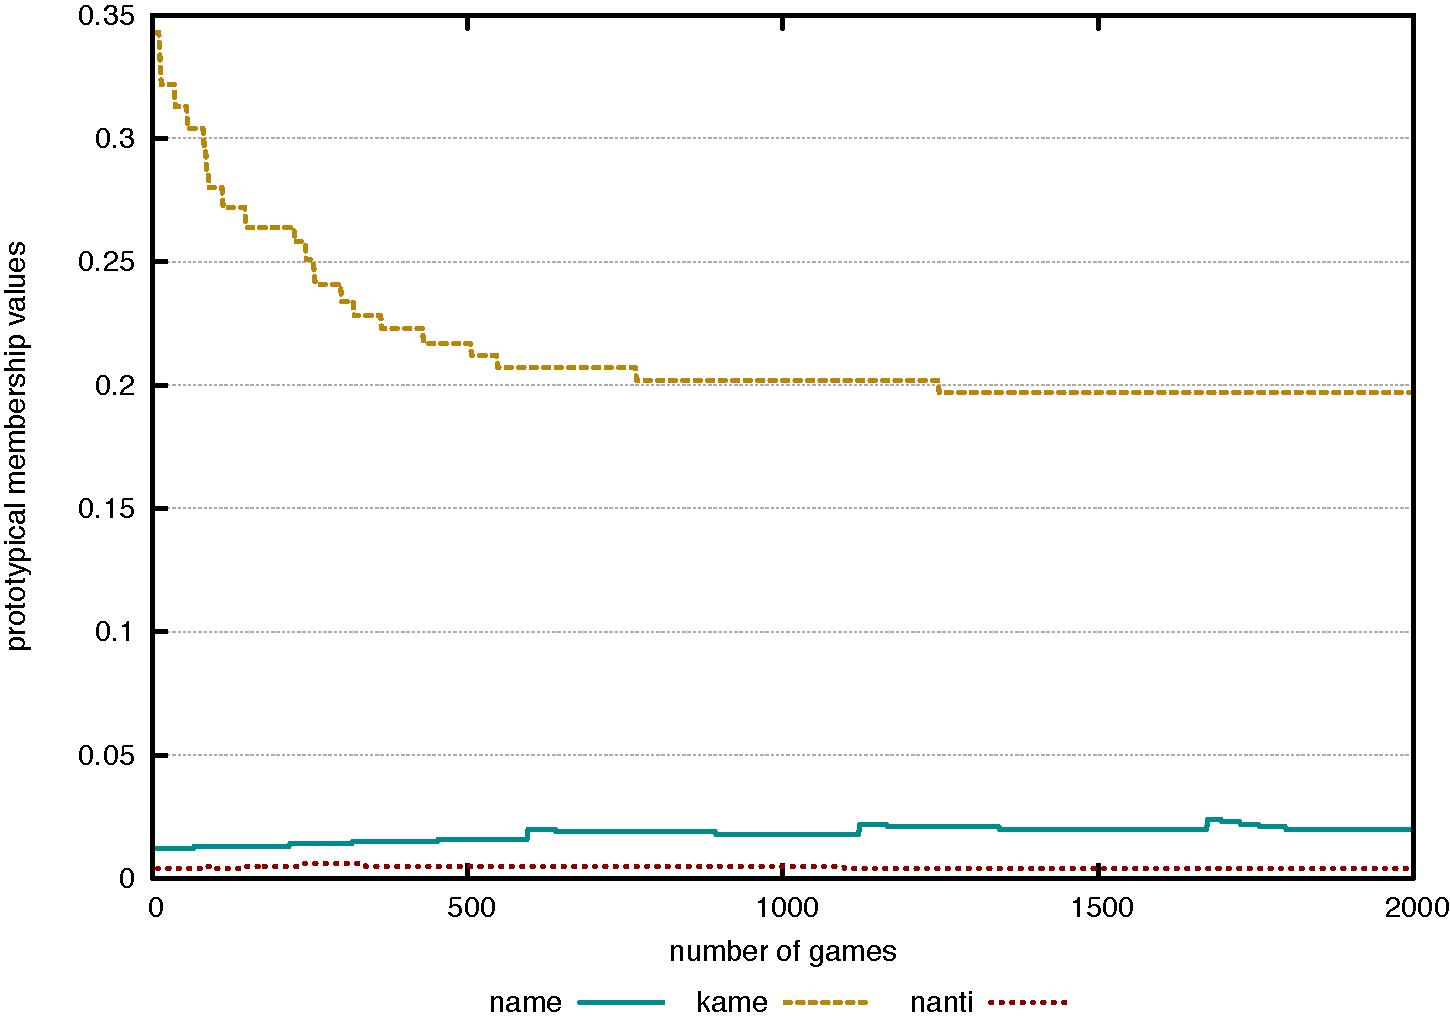
\includegraphics[width=.8\textwidth]{./graded-membership/figures/strict-acquisition-values.pdf}
    \caption[Prototypical membership values learned in an acquisition
    experiment]{Prototypical membership values learned in an
      acquisition experiment based on the Tarahumara language
      system. Initially, the prototypical membership values of these
      categories are quite different from the teacher. After around
      1000 interactions, the values approach those of the teacher
      until they match almost perfectly.}
    \label{f:gm-acquisition-values}
  \end{center}
\end{figure}

\section{Invention operator}

The invention operator 
\is{learning operators!invention operator!for graded membership strategy} 
can be triggered whenever a
speaker is not able to discriminate the colour of the randomly selected
topic. Whenever this occurs, the agent can extend the current language
system with a new membership category based on the membership value
of the topic of the current interaction. The rate at which an agent
chooses to do so, is controlled by the \textsc{membership category
  invention rate}
\is{invention rate!membership category}
\is{membership category invention rate|see{invention rate}}.
The lower this rate, the lower the chance of an agent inventing a new
membership category.

\subsection{Formation experiment}
\is{formation experiment!for graded membership strategy}

The goal of the formation experiment is to let a population of agents
develop its own system of membership categories. As the use of these
categories depends on the use of basic colour categories, the set
of basic colour categories is assumed to be shared within the
population, before they start inventing membership categories. 

The formation experiment is run in two different environments: an
unconstrained one and a constrained one. Unconstrained contexts consist of
five randomly drawn Munsell chips \citep{newhall42final}. Constrained
contexts will be introduced later on. The basic colour
category system that is shared by all agents at the onset of the
experiment is based on the Tarahumara language system (but without the
membership categories). The invention rate is set to 0.005.

\subsection{Measures}

\subsubsection{Number of membership categories}\todo{rename this chapter to: 8.2.2 "Measures of numbers of membership categories" ?}

\is{measures!number of membership categories}
\is{number of membership categories|see{measures}}

The number of membership categories of an agent ($n_{mc}$) simply
corresponds to the number of membership categories known to this
agent. At the level of a population $P$, it is understood as the
average number of known membership categories over all agents in the
population.

\begin{equation}
n_{mc}(P) = \frac{\displaystyle \sum_{i=1}^{|P|} n_{mc}(a)}{|P|}
\label{eq:number-of-membership-categories-population}
\end{equation}

\subsection{Results}

The resulting dynamics of the experiment in an unconstrained
environment are shown in Figure \ref{f:gm-formation-dynamics}. The
agents reach a level of communicative success that is higher than the
baseline experiment. The variance between the membership values of the
membership categories between agents is quite low. The higher level of
communicative success comes at the cost of a higher number of
membership categories (around 13 where in the baseline experiment
there were only 3). Moreover, this number does not seem to stabilise.

\begin{figure}[htpb]
  \begin{center}
    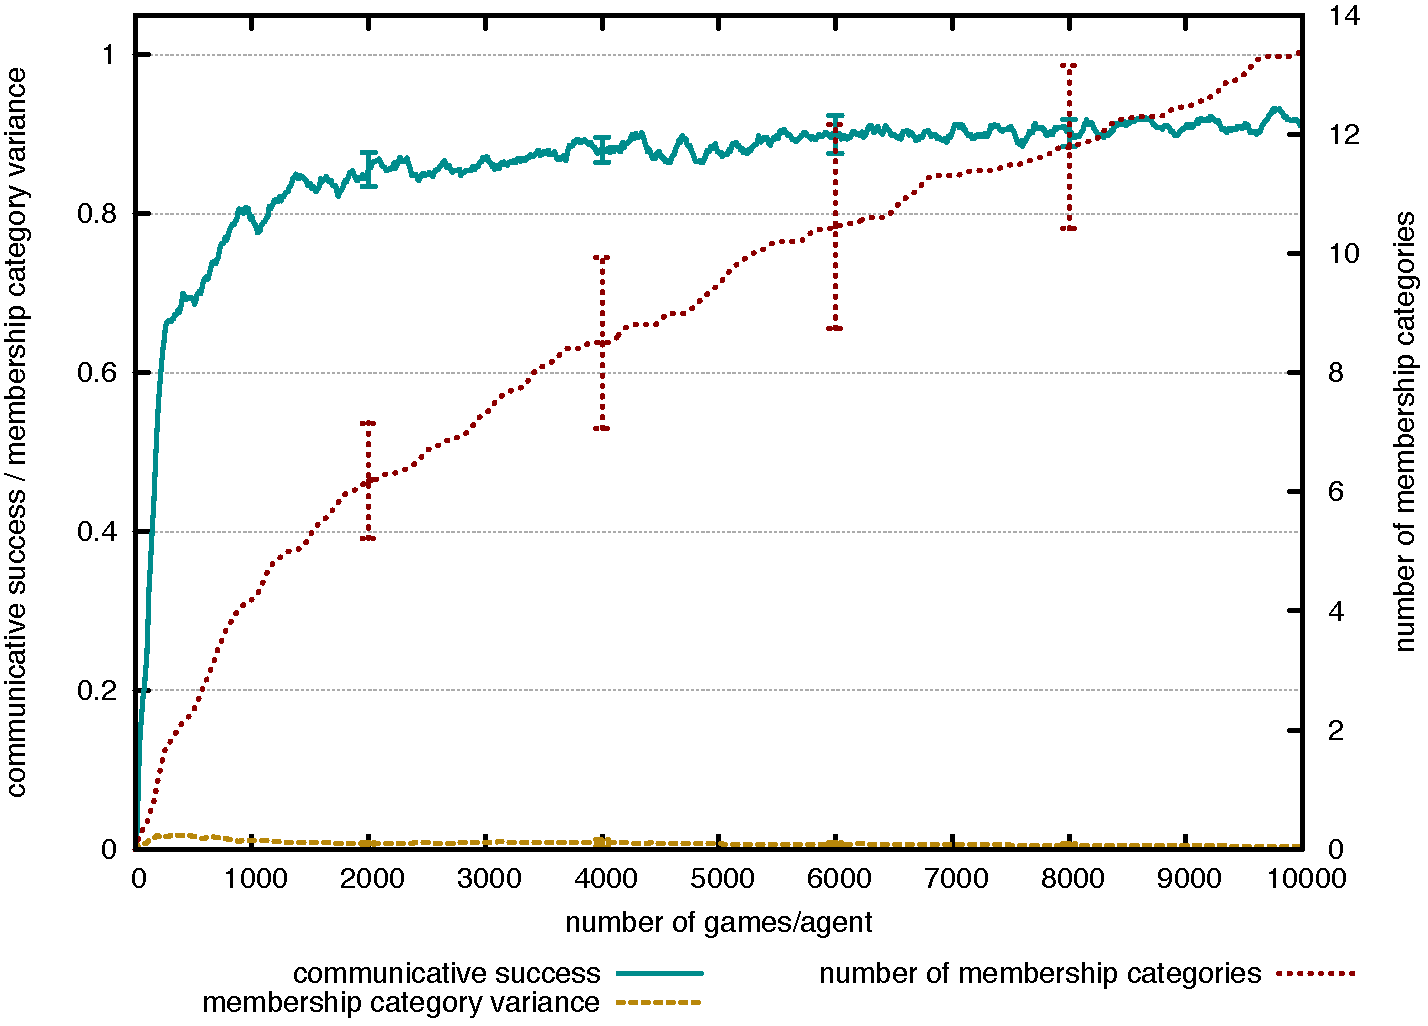
\includegraphics[width=.8\textwidth]{./graded-membership/figures/strict-formation.pdf}
    \caption[Dynamics of the formation experiment in an unconstrained
    environment]{Dynamics of the formation experiment in an
      unconstrained environment. The agents reach a level of
      communicative success that is higher than the baseline
      experiment, but this comes at the cost of a higher number of
      membership categories. The results are averaged over 10
      independent runs.}
    \label{f:gm-formation-dynamics}
  \end{center}
\end{figure}

\begin{figure}[htpb]
  \begin{center}
    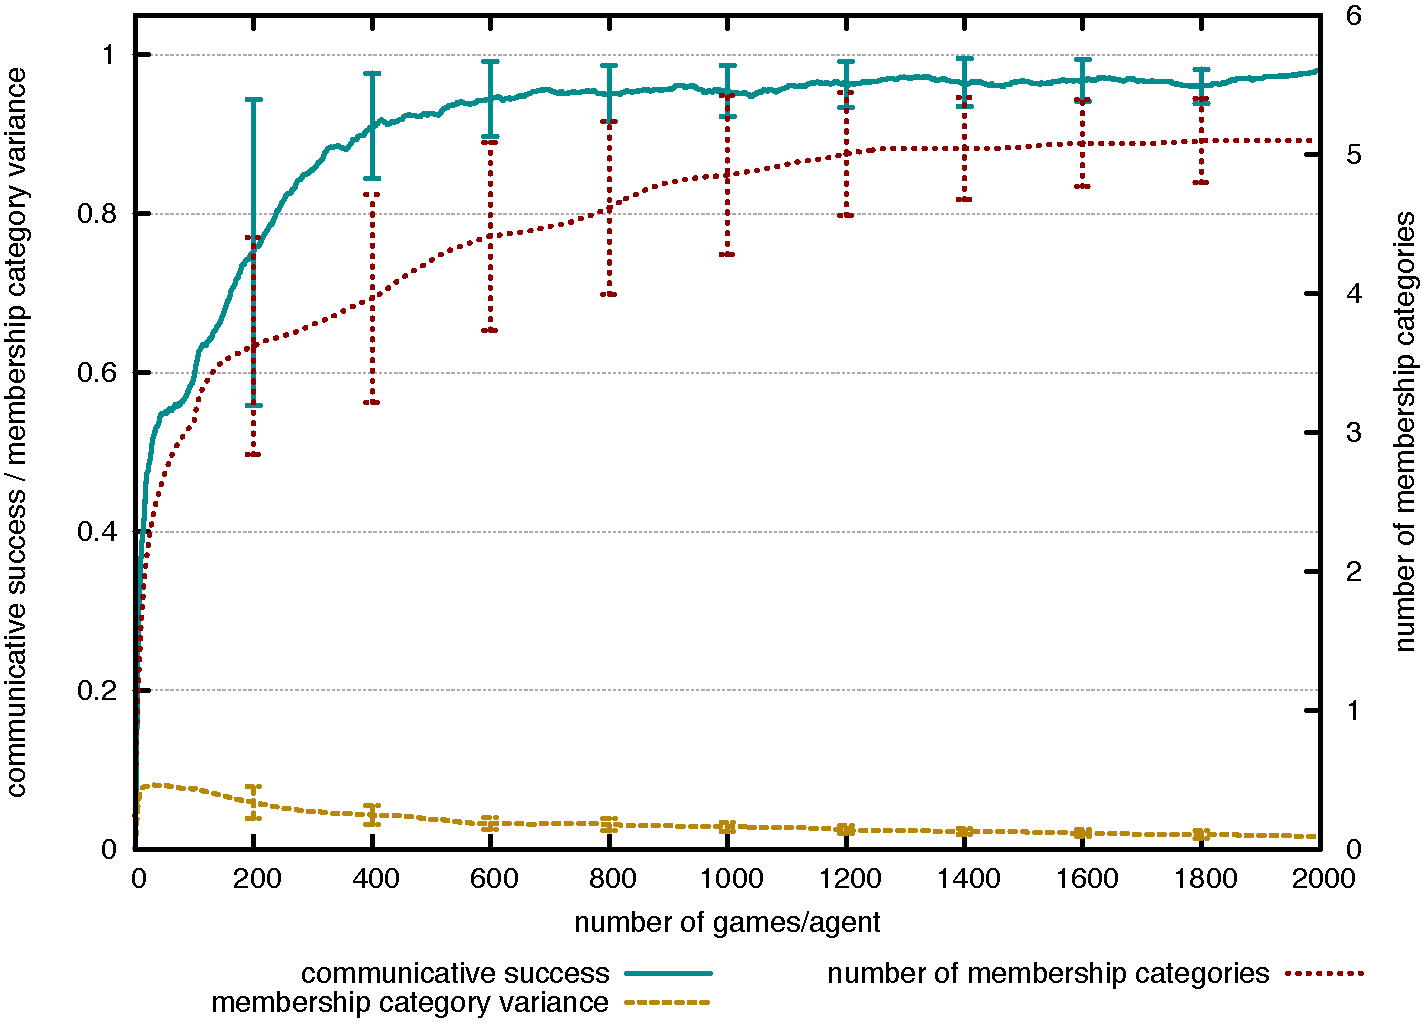
\includegraphics[width=0.8\textwidth]{./graded-membership/figures/strict-formation-constrained.pdf} % textwidth is set to prevent 2 additional pages for this chapter
    \caption[Dynamics of the formation experiment in a constrained
    environment]{Dynamics of the formation experiment in a
      constrained environment in which the difference in membership
      values of entities categorised as the same basic colour
      categories is guaranteed to be more than 0.2. This additional
      constraint results in a stable number of membership
      categories. The results are averaged over 10 independent runs.}
    \label{f:gm-formation-constrained-dynamics}
  \end{center}
\end{figure}

The main reason why the agents keep inventing new membership
categories in an unconstrained environment, is due to the continuous
nature of the membership function. Agents keep on encountering
situations in which their current repertoire of membership categories
is insufficient to discriminate the topic based on its membership
value. 

In order to verify this hypothesis, I have run exactly the same
model but now in a constrained environment: the difference between the
membership values of entities that belong to the same basic colour
categories is guaranteed to be above a certain threshold, which is set
to 0.2. As the agents are expected to invent only a limited number of
membership categories, the invention rate is set to 0.5.

The resulting dynamics are shown in Figure
\ref{f:gm-formation-constrained-dynamics}. The communicative success
reached by the agents is higher than in the previous experiment and
the membership variance is slightly higher than before. Most
importantly the average number of membership categories stabilises
around 5. This number corresponds exactly to the expected number of
required membership categories, as the membership function ranges from
zero to unity and a minimal difference of 0.2 in membership value is
guaranteed.



\section{Conclusion}

In this chapter, I have shown how the methodology that was used for
completing the basic colour strategy can readily be extended to cover
other language strategies, such as the graded membership strategy. I
have introduced the adoption and alignment operators that allow one
agent to pick up the membership categories used by another agent. The
performance of these operators is evaluated in an acquisition
experiment. Finally, I introduced the invention operator for the graded
membership strategy, which allows a population of agents to invent and
coordinate its own system of membership categories.